\documentclass[a4paper,10pt]{article}

\usepackage[margin=3cm]{geometry}
\usepackage{cmap}
\usepackage[T2A]{fontenc}
\usepackage[utf8]{inputenc}
\usepackage[english, russian]{babel}
\usepackage{hyperref, array, xcolor, listings, amsmath, ragged2e, forest}
\usepackage{amsmath}
\usepackage{listings}
\usepackage{graphicx}
\graphicspath{{./pictures/}}

\title{Конспекты по проге 1 семестр}
\author{{Никита Евсюков} {Маргарита Сагитова}}
\date{}

\begin{document}
	\maketitle
	\tableofcontents
	\newpage
	
	\section{Введение}
	\subsection{Алгоритм}
	\paragraph{Определение}
		Алгоритм ― это формально описанная вычислительная процедура, получающая исходные данные (input), называемые также входом алгоритма или его аргументом, и выдающая результат вычисления на выход (output).
		Алгоритм определяет функцию (отображение):
		\begin{equation}
			F \colon X \to Y
		\end{equation}
		$X$ - входные данные, $Y$ - выходные
	\paragraph{Примеры}
	\begin{center}
	Вычисление числа Фибоначчи
	\end{center}
	\begin{lstlisting}
		int fib(int n) {
			int x = 1;
			int y = 0;
			
			for (int i = 0; i < n; i++) {
				x += y;
				y = x - y;
			}
			return y;
		}
	\end{lstlisting}
	Или же через перемножение матриц за $O(log(n))$
	\[
	\begin{pmatrix}
		F_{0} & F_{1}
	\end{pmatrix}
	\begin{pmatrix}
		0 & 1 \\
		1 & 1
	\end{pmatrix} ^ {\!\!n}
	=
	\begin{pmatrix}
		F_{n} & F_{n+1}
	\end{pmatrix}
	\]

	\begin{center}
		Проверка числа на простоту
	\end{center}
	Перебор до $\sqrt{n}$ \\
	Решето Эратосфена
	
	\begin{center}
		Быстрое возведение в степень
	\end{center}
	\begin{lstlisting}
		int power (int a, int n) {
			if (n == 0) return 1;
			if (n % 2 == 0) {
				int b = power (a, n/2);
				return b*b;
			} else {
				return power (a, n - 1)*a;
			}
		}
	\end{lstlisting}
	\newpage
	\subsection{Асимптотики}
	$f$ ограничена сверху функцией $g$ асимптотически
	\[
		f(x) \in O(g(x)) \Leftrightarrow \exists (C>0)  (\forall x) \colon \| f(x) \| \leq C \| g(x) \|
	\]
	$f$ ограничена снизу функцией $g$ асимптотически
	\[
		f(x) \in \Omega(g(x)) \Leftrightarrow \exists (C>0)  (\forall x) \colon \| f(x) \| \geq C \| g(x) \|
	\]
	$f$ ограничена сверху и снизу функцией $g$ асимптотически
	\[
		f(x) \in \Theta(g(x)) \Leftrightarrow \exists (C > 0),(C' > 0) (\forall x) \colon C \|g(x)\| \leq \|f(x)\| \leq C' \|g(x)\|
	\]
	$g$ доминирует над $f$ асимптотически
	\[
		f(x) \in o(g(x)) \Leftrightarrow \forall(C > 0) (\forall x) \colon \| f(x) \| < C \| g(x) \|
	\]
	$f$ доминирует над $g$ асимптотически
	\[
		f(x) \in \omega(g(x)) \Leftrightarrow \forall(C > 0) (\forall x) \colon \| f(x) \| > C \| g(x) \|
	\]
	$f$  эквивалентна $g$ асимптотически при $n \rightarrow n_0$
	\[
		f(n) \sim g(n) \Leftrightarrow \lim_{n \to n_0} \frac{f(n)}{g(n)} = 1
	\]
	
	\begin{center}
		Примеры \\
		$O(1) = O(2)$ \\
		$O(f(n))O(g(n)) = O(f(n)g(n))$ \\
		$f(n) \subset g(n) \Rightarrow O(f(n) + g(n)) = O(g(n))$
	\end{center}
	
	\subsection{Структура данных, абстрактный тип данных (интерфейс)}
	\paragraph{Определение} Структура данных - программная единица, позволяющая хранить и обрабатывать данные. Для взаимодействия предоставляет интерфейс.
	\begin{center}
		Примеры \\
		int a[n]; \\
		std::pair<int, int> \\
	\end{center}
	Абстрактный тип данных (АТД) - тип данных, который скрывает внутреннюю реализацию, но предоставляет весь интерфейс для работы с данными, а также возможность создавать элементы этого типа. Абстрактный тип данных реализуется с помощью структуры данных.
	\begin{center}
		Пример \\
		Стек, реализованный через массив \\
		Стек - АТД, массив - структуры данных
	\end{center}
	\newpage
	\subsection{Массив}
	\paragraph{Определение} Массив - структура данных, хранящая набор значений (элементов), которые идентифицируются по индексу или набору индексов. \\
	Динамический массив - массив, размер которого может изменяться во время выполнения программы. \\
	
	Линейный поиск - поиск по массиву за $O(n)$ \\
	В отсортированном массиве поиск возможен за $O(log(n))$ с помощью бинарного поиска \\
	\begin{lstlisting}
		int binarySearch(const int *a, int n, int item) {
    			int leftPtr = -1, rightPtr = n;

			 while (rightPtr - 1 > leftPtr) {
				int middlePtr = (leftPtr + rightPtr)/2;
				if (item > a[middlePtr]) {
					leftPtr = middlePtr;
				} else if (item < a[middlePtr]) {
					rightPtr = middlePtr;
				} else {
					return middlePtr;
				}
			}
			return rightPtr;
		}
	\end{lstlisting}
	\newpage
	\section{Базовые структуры данных}
	\subsection{Динамический массив}
	$+\colon$ random access operator \\
	$-\colon$ нельзя удалить/вставить в середину за $O(1)$
	\subsection{Односвязный и двусвязный список}
	$+\colon$ удаление и вставка в любое место \\
	$-\colon$ поиск/последовательный доступ дорог \\
	Односвязный список имеет ссылку только на следующий узел. \\
	Двусвязный список имеет ссылку на следующий и предыдущий узлы. \\
	\begin{center}
		Операции со списками: \\
		\item Поиск элемента ($O(n)$)
		\item Вставка - смена указателей ($O(1)$)
		\item Удаление - смена указателей ($O(1)$)
		\item Объединение (при условии, что храним указатель на последний элемент) - смена указателей ($O(1)$)
	\end{center}
	\subsection{Стек}
		Сертификат - Last In First Out \\
	\begin{center}
		Операции: \\
		\item Добавление в конец ($O(1)$)
		\item Удаление с конца ($O(1)$)
	\end{center}
	\begin{center}
		Можно реализовать с помощью: \\
		\item Динамического массива
		\item Списка
	\end{center}
	Для хранения в массиве можно использовать указатель на последний элемент и сдвигать его в зависимости от операции. \\
	Чтобы поддерживать минимум в стеке, достаточно хранить не элемент, а пару вида: значение элемента, минимальный элемент в стеке на момент вставки нашего элемента. \\
	\subsection{Очередь}
		Сертификат - First In First Out \\
	\begin{center}
		Операции: \\
		\item Добавление в конец
		\item Удаление из начала
	\end{center}
	\begin{center}
		Можно реализовать с помощью: \\
		\item Динамического массива
		\item Списка
		\item Двух стеков
	\end{center}
	\begin{center}
		Циклическая очередь в массиве
	\end{center}
	Реализация циклической очереди в массиве основана на хранении двух указателей: на первый элемент в очереди и на последний. Тогда удаление/вставка элементов будет связана со сдвигом указателя на первый/последний элемент по формуле newPtr = (ptr + 1)\%size \\
	\begin{center}
		Хранение очереди в списке
	\end{center}
	Для реализации на односвязном списке достаточно хранить указатель на первый и последний элемент, удаление/вставка производятся сменой указателей. \\
	\begin{center}
		Представление очереди в виде двух стеков
	\end{center}
	Для реализации очереди на двух стеках достаточно вставлять элементы в один стек, а забирать из другого. В случае, если второй стек пуст, перемещать все элементы из первого во второй. \\
	\begin{center}
		Время извлечения элемента
	\end{center}
	Для операции push возьмём 3 монеты: для самого push'а, резерв на pop из первого стека и резерв на pop из второго. Тогда учётная стоимость pop'а из второго стека будет равна 0, т.к. можно использовать оставшиеся монеты. Таким образом, каждая операция за $O(1)$ \\
	\begin{center}
		Поддержка минимума в очереди
	\end{center}
	Для поддержки минимума необходимо поддерживать минимум в каждом из стеков, тогда минимум в очереди - меньший минимум стеков. \\
	\subsection{Дек}
		Список элементов, в котором можно вставлять и удалять элементы с конца и начала.
	\begin{center}
		 Операции: \\
		 \item Вставка в конец
		 \item Извлечение из конца 
		 \item Вставка в начало
		 \item Извлечение из начала
	\end{center}
	\begin{center}
		 Можно реализовать с помощью: \\
		 \item Динамический массива
		 \item Двусвязного списка
	\end{center}
	\begin{center} 
		Хранение дека в массиве
	\end{center}
	Хранение аналогично очереди, только указатели могут сдвигаться как вперёд, так и назад (newPtr = (ptr - 1)\%size)
	\begin{center}
		Хранение дека в списке
	\end{center}
	Храним аналогично очереди, но используем двусвязный список. \\
	\subsection{Двоичная куча. АТД Очередь с приоритетом}
	\begin{center}
	\begin{forest}
		for tree={
			grow=south,
			circle, draw, minimum size=3ex, inner sep=1pt,
			s sep=7mm
			}
		[0(root)
			[1
				[3]
				[4]
			]
			[2
				[5]
				[6]
			]
		]
	\end{forest}
	\end{center}
	\paragraph{Определение}
	Двоичное подвешенное дерево, которое удовлетворяет свойствам:
	\begin{center}
		\item Значение в вершине $\leq$ ($\geq$ для максимума в корне) значению в потомке
		\item На $i$-ом слое $2^i$ вершин (кроме, возможно, последнего). Глубина кучи $\log{n}$
		\item Последний слой заполняется слева направо
	\end{center}
	\begin{center}
		Удобно хранить бинарную кучу в массиве: \\
		\item $a[0]$ - корень
		\item $a[i] \rightarrow (a[2i+1], a[2i+2])$ - потомки
	\end{center}
	\paragraph{Операции}
	Вставка за $O(\log{n})$:
	\begin{center}
		\item Вставляем в свободное место
		\item Рекурсивно поднимаем элемент, если он меньше (больше) родителя (siftUp)
	\end{center}
	Удаление за $O(\log{n})$:
	\begin{center}
		\item Удаляем минимум
		\item Вставляем последний элемент в корень
		\item Рекурсивно меняем элемент с минимальным (максимальным) потомком (siftDown)
	\end{center}
	\paragraph{Очередь с приоритетом}
	- абстрактный тип данных, который поддерживает следующие операции: 
	\begin{center}
		\item push - добавить в очередь элемент с определенным приоритетом
		\item pop - удалить из очереди элемент с наивысшим приоритетом
		\item top - посмотреть элемент с наивысшим приоритетом (необязательная операция)
	\end{center}
	\subsection{Амортизационный анализ}
	\paragraph{Определение}
	- метод подсчёта времени, требуемого для выполнения последовательности операций над структурой данных. При этом время усредняется по всем выполняемым операциям, и анализируется средняя производительность операций в худшем случае.
	\paragraph{Средняя амортизационная стоимость}
	\[
		x = \frac{\sum_{i=0}^{n} t_{i}}{n}
	\]
	$t_{i}$ - время выполнения $i$-ой операции
	\paragraph{Амортизированное (учетное) время добавления элемента в динамический массив}
	Стоимость операции add(item) \\
	Для каждой операции add(item), для которой не требуется расширение массива, будем использовать три монетки: одна для самой вставки, две в резерв. Одну из резерва положим к вставленному элементу с индексом $i$, а вторую к элементу с индексом $i - \frac{n}{2}$, где $n$ - размер массива\\
	Когда массив заполнится, у каждого элемента будет одна монетка в резерве, которую мы сможем использовать для копирования в новый массив размером $2n$ \\
	\paragraph{Метод потенциалов}
	Пусть $\Phi$ - потенциал \\
	$\Phi_{0}$ - изначальное значение \\
	$\Phi_{i}$ - состояние после $i$-ой операции \\
	Тогда стоимость $i$-й операции $a_{i} = t_{i} + \Phi_{i} - \Phi_{i-1}$ \\
	Пусть $n$ - количество операций, $m$ - размер структуры данных, тогда $a = O(f(n,m))$, если: \\
	\begin{center}
		\item $\forall i \colon a_{i} = O(f(n,m))$
		\item $\forall i \colon \Phi_{i} = O(n(f(n,m)))$
	\end{center}
	Доказательство \\
	\[
		a = \frac{\sum_{i=1}^{n} t_{i}}{n} = \frac{\sum_{i = 1}^{n} a_{i} + \sum_{i = 0}^{n-1} \Phi_{i} - \sum_{i = 1}^{n} \Phi_{i}}{n} = \frac {n \cdot O(f(n,m)) + \Phi_{0} - \Phi_{n}}{n} = O(f(n,m))
	\]
	\paragraph{Метод бух. учёта}
	Пусть операция стоит некоторое число монет. \\
	Тогда для каждой операции мы можем взять монет с запасом, чтобы хватило на следующие возможные операции (пример с динамическим массивом) \\
	Если монет хватило на все операции, то наше предположение о стоимости каждой операции (то, что мы взяли с запасом) верно \\
	(Излагаю в неформальном стиле) \\
	\subsection{Персистентный стек}
	Стек, который хранит все свои состояния \\
	Операции:
	\begin{center}
		\item Вставка: $push(i,x) \rightarrow j$, где $i$ - конкретное состояние, $x$ - элемент, который нужно вставить, $j$ - новое состояние после вставки. При вставке создаётся новое состояние стека, где хранится вставленный элемент и ссылка на состяоние, в которое его вставили.
		\item Удаление: $pop(i) \rightarrow j$. При удалении $i$ - ого состояния идём с "родителю" $i$-ого состояния и подцепляем его копию к "деду" $i$-ого состояния.
	\end{center}
	В итоге имеем доступ к любой версии стека за $O(1)$ времени и $O(n)$ памяти. \\
	Можно реализовать с помощью:
	\begin{center}
		\item Массива
		\item Списка
	\end{center}
	\section{Сортировки и порядковые статистики}
	\subsection{Задача сортировки, устойчивость, локальность}
	\paragraph{Задача} - упорядочить множества объектов по какому-либо признаку \\
	\begin{center} 
		\textbf{Классификация} 
	\end{center}
	\begin{itemize}
		\item По времени работы
		\item По количеству дополнительной памяти
		\item Устойчивость - сортировка не меняет порядок объектов с одинаковыми ключами
		\item Локальность - сортировка в том же контейнере
		\item Детерменированность - каждая операция присваивания, обмена и т.д. не зависит от предыдущих
	\end{itemize}
	\subsection{Квадратичные сортировки}
	Пузырьки там всякие \\
	\subsection{Сортировка слиянием}
	\begin{itemize}
		\item Сложность - $O(n\log n)$
		\item Дополнительная память - $O(n)$
	\end{itemize}
	\paragraph{Принцип} - разделяем массив на подмассивы, сортируем их рекурсивно, сливаем
	\subsection{Сортировка с помощью кучи}
	\begin{itemize}
		\item Сложность - $O(n\log n)$
		\item Дополнительная память - $O(1)$
	\end{itemize}
	\paragraph{Принцип} - последовательно меняем корень с последним элементом и уменьшаем размер на 1
	\subsection{Слияние отсортированных массивов с помощью кучи}
	\begin{itemize}
		\item Сложность - $O(q\log k)$, где $q$ - суммарная длина всех массивов, $k$ - количество массивов
		\item Дополнительная память - $O(k)$
	\end{itemize}
	\begin{center}
		\textbf{Принцип}
	\end{center}
	\begin{itemize}
		\item Делаем кучу на $k$ элементов
		\item Сдвигаем указатель минимального элемента и добавляем его в новый массив
		\item Добавляем элемент по новому указателю в кучу
	\end{itemize}
	\subsection{Нижняя оценка времени работы для сортировок сравнением}
	Сопоставим алгоритм сортировки с деревом, в котором листья - конечные перестановки исходного массива, узлы - операции сравнения, а рёбка - переходы между состояниями алгоритма, докажем, что высота такого дерева не меньше чем $\Omega(n \log n)$, где $n$ - количество элементов \\
	\textbf{Доказательство} \\
	Число листьев не меньше общего количества перестановок - $n!$ \\
	С другой стороны, двоичное дерево имеет не более $2^n$ перестановок \\
	\[
		n! \leq 2^h \Leftrightarrow h \geq \log_2 n! > \frac{n}{2}*\log_2(\frac{n}{2}) = \frac{n}{2}(\log_2 n - 1) = \Omega(n \log n)
	\]
	\subsection{Быстрая сортировка}
	\paragraph{Принцип}
	Есть массив $a[0...n-1]$ и некоторый подмассив $a[l..r]$
	\begin{center}
		\item Разделим $a[l...r]$ на две части по опорному элементу $q$: $a[l...q]$ и $a[q+1...r]$ так что каждый элемент $a[l...q]$ меньше или равен $a[q]$, который не превышает любой элемент подмассива $a[q+1...r]$
		\item Подмассивы $a[l...q]$ и $a[q+q...r]$ сортируются с помощью рекурсивного вызова быстрой сортировки
	\end{center}
	\paragraph{Схема Ломуто}
	\begin{center}
		\item Выбираем $q = a[r]$
		\begin{lstlisting}
			q = a[r];
			i = l;
			for (int j = l; j < r - 1, j++) {
				if (a[j] < q) {
					swap(a[i], a[j]);
					i++;
				}
			}
			swap(a[i], a[r];
		\end{lstlisting}
	\end{center}
	\newpage
	\paragraph{Схема Хоара}
	\begin{center}
		\begin{lstlisting}
			q = A[(r + l)/2];
			i = l;
			j = r;
			while (i <= j) {
				while (a[i] < q) {
					i++;
				}
				
				while (a[j] > q) {
					j--;
				}
				if (i >= j) {
					break;
				}
				swap(a[i], a[j]);
				i++;
				j--;
			}
		\end{lstlisting}
	\end{center}
	\paragraph{Свойства}
	\begin{itemize}
		\item Локальная
		\item Недетерминированная
		\item Неустойчивая
	\end{itemize}
	\paragraph{Асимптотика}
	Дерево рекурсий
	\begin{center}
	\begin{forest}
		for tree={
			grow=south,
			circle, draw, minimum size=3ex, inner sep=1pt,
			s sep=7mm
			}
		[n
			[n/2
				[...
					[1]
				]
				[...
					[1]
				]
			]
			[n/2
				[...
					[1]
				]
				[...
					[1]
				]
			]
		]
	\end{forest}
	\end{center}
	\[
		T(n) = 2T(\frac{n}{2}) + O(n)
	\]
	Худший случай: $T(n) = T(n-1) + \Theta(n)$ (закинули один элемент от partitional) \\
	\[ 
		T(n) = \sum_{k = 1}^{n} \Theta(k) = \Theta(\sum_{k=1}^{n} k) = \Theta(n^2) 
	\]
	\newpage
	\paragraph{Среднее время работы}
	$O(n\log{n})$
	\paragraph{Доказательство}
	Пусть $X$ - суммарное количество операций сравнения с опорным элементом. Рассмотрим массив
	$[z_{0}...z_{n}]$, пусть $z_{ij} = [z_{i}...z_{j}]$ \\
	Опорный элемент дальше не участвует в сравнении $\Rightarrow$ сравнение каждой пары $\leq$ 1 раза \\
	\[
	X = \sum_{i=1}^{n-1} \sum_{j=i+1}^{n} X_{ij}
	\] 
	где $X_{ij} = 1$, если произошло сравнение $z_{i}$ и $z_{j}$, иначе 0 \\
	Применим мат. ожидание к каждой части
	\[ 
	E[X] = E[\sum_{i=1}^{n-1} \sum_{j=i+1}^{n} X_{ij}] = \sum_{i=1}^{n-1} \sum_{j=i+1}^{n} E[X_{ij}] = \sum_{i=1}^{n-1} \sum_{j=i+1}^{n} Pr(z_{i}, z_{j})
	\]		
	где $Pr(z_{i}, z_{j})$ - вероятность того, что $z_{i}$ сравнивается с $z_{j}$ \\
	Пусть все элементы различны \\
	$x$ - опорный $\Rightarrow (\forall z_{i}, z_{j} \colon z_{i} < x < z_{j} \Rightarrow$ $z_{i}$ и $z_{j}$ не будут сравниваться)  \\
	Если $z_{i}$ - опорный, то он сравнивается с каждым элементом $z_{ij}$ кроме себя \\
	Значит $z_{i}$ и $z_{j}$ будут сравниваться, когда первым в $z_{ij}$ будет выбран один из них \\
	$X_{ij} = 1 \Leftrightarrow z_{i}$ - опорный или $z_{j}$ - опорный
	\[ 
	Pr(z_{i}, z_{j}) = Pr(z_{i}) + Pr(z_{j}) = \frac{1}{j-i+1} + \frac{1}{j-i+1} = \frac{2}{j-i+1}
	\]
	где $Pr(z_{i})$ - вероятность того, что первым элементом был $z_{i}$, а $Pr(z_{j})$ - вероятность того, что первым был $z_{j}$, тогда
	\[
	E[X] =  \sum_{i=1}^{n-1} \sum_{j=i+1}^{n} \frac{2}{j-i+1}
	\]
	Пусть $k = j - i$, тогда
	\[
	E[X] =  \sum_{i=1}^{n-1} \sum_{k=1}^{n-i} \frac{2}{k+1} = \sum_{i=1}^{n-1} \sum_{k=1}^{n-i} \frac{2}{k} = \sum_{i=1}^{n-1} O(\log{n}) = O(n\log{n})
	\]
	\paragraph{Улучшения быстрой сортировки}
	\begin{itemize}
		\item Выбор медианы из первого, среднего и последнего элементов и отсечение рекурсии меньших подмассивов (с помощью сортировок вставками)
		\item Разделение на три части (применяют, если много одинаковых элементов)
	\end{itemize}
	\subsection{$k$ порядковая статистика}
	В чём суть: пусть дан массив A длиной N и пусть дано число K. Задача в том, чтобы найти в этом массиве K-ое по величине число, т.е. K-ую порядковую статистику
	\paragraph{Алгоритм}
	Пусть опорный элемент имеет индекс m \\
	Если $k == m$ $\Rightarrow$ успех \\
	Если $k < m \Rightarrow$ ищем k-ую статистику в левой части \\
	Если $k > m \Rightarrow$ ищем (k - m - 1)-ую статистику в правой части \\
	\paragraph{Асимптотика}
	Функция partition при поиске в массиве размера $n$ делает не более $n-1$ сравнений \\
	Проведём оценку сверху, будем считать, что каждый раз выбирается большая половина \\
	\[
		T(n) \leq \frac{1}{n} \sum_{k=1}^{n} (T(max(k-1; n - k) + n - 1) = n - 1 + \frac{1}{n} \sum_{k=1}^{n} (T(max(k-1; n - k)) = n - 1 + \frac{2}{n}\sum_{k = \lfloor n/2 \rfloor}^{n-1} T(k)
	\]
	Доказательство по индукции, пусть $T(k) \leq ck$ для константы $c \geq 4$ и всех $k<n$
	База: $T(1) = 0 < 4$ \\
	Тогда верно:
	\[
		T(n) = n - 1 + \frac{2}{n}\sum_{k = \lfloor n/2 \rfloor]}^{n-1} ck
	\]
	Арифметическая прогрессия:
	\[
		\sum_{k = \lfloor n/2 \rfloor]}^{n-1} ck = \frac{1}{2}(\lceil \frac{n}{2} \rceil + c(n-1)) \leq \frac{c}{2}(\frac{n+1}{2} - 1) \frac{3n - 2}{2} = c \frac{n - 1}{4} \frac{3n - 2}{2}
	\]
	Тогда выражение для $T(n)$ принимает вид:
	\[
		T(n) \leq n - 1 + \frac{2c(n-1)(3n-2)}{n*4*2} = n - 1 + c \frac{n - 1}{2n} \frac{3n - 2}{2} \leq \frac{c}{4} (n-1) + \frac{c}{4}(\frac{n - 1}{n}*(3n - 2)) \leq \frac{c}{4}(n - 1 + 3n - 2) = \frac{c}{4}(4n - 3) \leq cn
	\]
	Таким образом $T(n) = O(n)$
	\subsection{Сортировка подсчётом}
	Пусть у нас n целых чисел в диапазоне от $0$ до $k$ \\
	Обычно применяют, если $n$ много больше $k$ \\
	\paragraph{Алгоритм}
	Заводим массив $A[k]$ \\
	Проходим по нашему изначальному массиву и инкрементируем $A[i]$, если встретили $i$ - ое число \\
	\\ В случае целых чисел просто будем сдвигать число при записи в массив, и сдвигать обратно при доступе к элементу \\
	Также можно сортироввть по ключам сложные объекты \\
	Предварительно подсчитывает количества элементов с различными ключами и разделяем результирующий массив на соответствующие блоки (длины которых как раз и равны значениям вспомогательного массива, который мы получили \\
	Затем при повторном проходе исходного массива каждый элемент копируется в специальнго отведенный его ключу блок \\
	\paragraph{Асимптотика}
	$O(n+k)$
	\subsection{Блочная сортировка}
	\paragraph{Суть сортировки}
	Блочная сортирвка применяется при равномерном распределении входных данных \\
	Т.е. мы разбиваем вхдные данные на $n$ блоков. Внутри блока же сортируем удобным образом (либо той же блочной сортировкой). Сортировка работает только в том случае, если разбиение на блоки производится таким образом, чтобы элементы каждого следующего блока были больше предыдущего
	\paragraph{Где же применяем?}
	Эту сортировку стоит применять в случае, если данные распределены равномерно, т.е. велика вероятность того, что числа редко повторяются (например, последовательность случайных чисел) \\
	\subsection{Поразрядная сортировка}
	\paragraph{Общий смысл}
	Сначала сравниваем крайний разряд, группируем элементы по значению разряда \\
	Потом сравниваем числа по следующему разряду (сравниваем внутри группы) \\
	Перед сортировкой необходимо привести все данные к единому количеству "разрядов"
	\paragraph{MSD}
	Сравниваем, начиная со старшего разряда \\
	Добавляем "пустые" элементы (когда приводим к одинаковому количеству разрядов) в конец \\
	Подходит для строк \\
	\paragraph{LSD}
	Сравниваем, начиная с младшего разряда \\
	Добавляем "пустые" элементы (когда приводим к одинаковому количеству разрядов) в начало \\
	Подходит для чисел \\
	Но необходима устойчивая сортировка каждого разряда \\
	\paragraph{Пример}
	\[
		\begin{pmatrix}
			32[9] \\
			45[6] \\
			43[7] \\
		\end{pmatrix}
		\rightarrow
		\begin{pmatrix}
			32[9] \\
			43[7] \\
			45[6] \\
		\end{pmatrix}
		\rightarrow
		\begin{pmatrix}
			32[9] \\
			43[7] \\
			45[6] \\
		\end{pmatrix}
		\rightarrow
		\begin{pmatrix}
			3[2]9 \\
			4[3]7 \\
			4[5]6 \\
		\end{pmatrix}
		\rightarrow
		\begin{pmatrix}
			[3]29 \\
			[4]37 \\
			[4]56 \\
		\end{pmatrix}
	\]	
	\paragraph{Асимптотика LSD}
	Пусть $m$ - количество разрядом \\
	$n$ - количество чисел \\
	$k$ - количество значений каждого разряда (10 для чисел) \\
	$T(n)$ - время работы устойчивой сортировки \\
	Тогда сложность $O(m(n+k))$, если устойчивая сортировка имеет сложность $O(n+k)$ (сортировка подсчётом, например)
	\paragraph{MSD для строк}
	По первому символу разделяем строки в кучи \\
	Каждую кучу делим аналогично \\
	Когда куча достигла размера 1 - элемент на месте
	\paragraph{Асимптотика MSD}
	Пусть значения разрядов меньше $b$, а количество разрядок - $k$ \\
	Если "делим хорошо" (разбиваем на разные кучки), асимптотика $\Omega(n\log_{b}n)$ \\
	Если "делим плохо" (например, возможна ситуация строк BBBBA и BBBBC), асимптотика $O(nk)$ \\
	\subsection{Бинарная быстрая сортировка}
	Аналог MSD сортировки для строк, но алфавит состоит только из 0 и 1 
	\subsection{Мастер-теорема}
	\paragraph{О чём?} Мастер теорема позволяет найти асимптотическое решение рекуррентных соотношений, которые могут возникнуть в анализе асимптотики многих алгоритмов.
	\paragraph{Формулировка} Пусть  $a \geq 1$ и $b > 1$ - константы, $f(n)$ - функция, $T(n)$ определено на множестве неотрицательных целых чисел как: 
	\[
		T(n) = a*T(\frac{n}{b}) + f(n)
	\], где $n$ - размер задачи \\
	$a$ - количество подзадач в рекурсии \\
	$n/b$ - размер каждой подзадачи \\
	$f(n)$ - оценка сложности работы вне рекурсии \\
	Пример для merge-sort 
	\[	
		T(n) = 2T(\frac{n}{2}) + f(n)
	\]	
	где $f(n)$ - затраты на слияние $(n)$\\
	\textbf{Тогда:}
	\begin{itemize}
		\item Если $f(n) = O(n^{\log_b a - \epsilon})$ для некоторого $\epsilon > 0$, то $T(n) = \Theta(n^{\log_b a})$
		\item Если $f(n) = \Theta(n^{\log_b a})$, то $T(n) = \Theta(n^{\log_b a} \log n)$
		\item Если $f(n) = \Omega(n^{\log_b a + \epsilon})$ для некоторого $\epsilon > 0$ и если $af(\frac{n}{b}) \leq cf(n)$ для некоторой константы $c < 1$ и всех достаточно больших $n$, то $T(n) = \Theta(f(n))$
	\end{itemize}
	По сути, большая из фукнций ($f(n)$ и $n^{\log_b a}$) определяет рекуррентное соотношение \\
	Доказательство в Кормене на 124 странице \\

\subsection{Сортировочные сети}
\begin{center}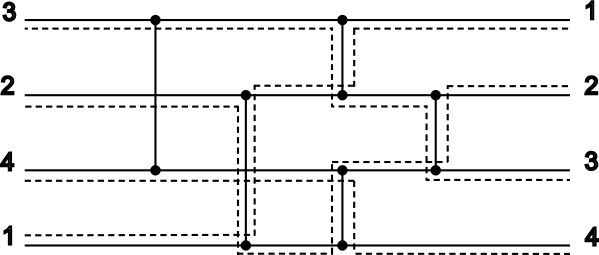
\includegraphics{snet1.png}\end{center}
\textbf{Сортирующая сеть} — метод сортировки, основанный только на сравнениях данных. Схематически изображается в виде параллельных прямых (проводов), соединенных вертикальными линиями (компараторами). Особенность сети сортировки в том, что сравнения выполняются независимо от предыдущих. Кроме того, сравнения могут выполняться одновременно.\\
\textbf{Компаратор} - устройство, подключенное к двум проводам, которое упорядочивает текущие значения на проводах. K-компаратор упорядочивает значения на k проводах.\\
\textbf{Глубина компаратора} - максимум из количества узлов на входных проводах.\\
\textbf{Слой сети} — множество компараторов, имеющих одинаковую глубину.\\
\textbf{Глубина сети}— количество слоев в сети.\\
\textbf{Размер сети} - количество компараторов в сети.\\
\paragraph{0-1 принцип} - позволяет проверять корректность работы сети за О($2^n \cdot Comp(n)$)\\
\paragraph{Теорема} Сеть компараторов с n входами является сортирующей тогда и только тогда, когда она сортирует $2^n$ различных последовательностей из 0 и 1.\\
\paragraph{Доказательство} Если функция f - монотонна, то $f(min(x_1, x_2)) = min(f(x_1, f(x_2))$\\
Пусть f - монотонная функция, а N - сеть компараторов, докажем, что они коммутируют, т.е f(N(a)) = N(f(a)), где а - последовательность $\{a_1, a_2, ..., a_n\}$, a $f(a)=\{f(a_1), ..., f(a_n)\}$\\
Рассмотрим компаратор C, сортирующий эдементы i и j. С(i) = min(i, j), тогда f(C(i)) = f(min(i, j)) = min(f(i), f(j)) = C(f(i)).\\
Таким образом, результат не зависит от того, что мы сделаем с отдельным компаратором сначала: применим монотонную функцию или пропустим его через сеть. Те же рассуждения можно провести для всех других индексов, то есть для всей сети тоже верно.\\
\textbf{Сам принцип} - Пусть сеть N сортирует $a_1, ..., a_n$ в возрастающем порядке и есть последовательность а, которую она не сортирует, тогда найдется такое i, $N(a_i) > N(a_{i+1}$.\\
Рассмотрим функцию $f(x) = \begin{cases} 0, x < N(a_i) \\ 1, x \geq N(a_i) \end{cases}$\\
Она монотонна и f($N(a_i)$) = 1, a  f($N(a_{i+1})$) = 0, то есть f(N(a)) не отсортирована. Значит и N(f(a)) - не отсортирована, но по предположению теоремы все последовательности из нулей и единиц сеть сортирует правильно, что приводит к противоречию, значит такой последовательности а, которую сеть не сортирует не существует.\\
\subsection{Сеть Бетчера}
Сеть Бетчера (англ. Batcher bitonic mergesort) — сортирующая сеть размером O(n$log^2$n) и глубиной O($log^2$n), где n — число элементов для сортировки. Здесь рассматривается случай, когда n = $2^k$\\
\paragraph{Битоническая последовательность} - конечный упорядоченный набор (кортеж) из вещественных чисел, в котором они сначала монотонно возрастают, а затем монотонно убывают, или набор, который приводится к такому виду путем циклического сдвига.\\
Приведем несколько примеров нуль-единичной битонической последовательности: 00111000, 11000111, 1110, 1, 000.
\paragraph{Битонический сортировщик} - эффективно сортирует все битонические последовательности.\\
Битонический сортировщик представляет собой каскад так называемых полуфильтров. Каждый полуфильтр — сеть компараторов единичной глубины, в которой i-й входной провод сравнивается со входным проводом с номером $\frac{n}{2}$+i, где i=1,2,…,$\frac{n}{2}$ (число входов n — чётное).\\
\paragraph{Лемма} Если на вход в полуфильтр подать битоническую последовательность из нулей и единиц длиной n, то на выходе мы получим две битонические последовательности длиной $\frac{n}{2}$ такие, что каждый элемент из верхней последовательности не превосходит любой элемент из нижней, и что одна из них будет однородной (англ. clean) — целиком состоящей либо из нулей, либо из единиц.\\
\textbf{Доказательство}  без ограничения общности для случая, когда последовательность имеет вид 0..01..10..0\\
\begin{center}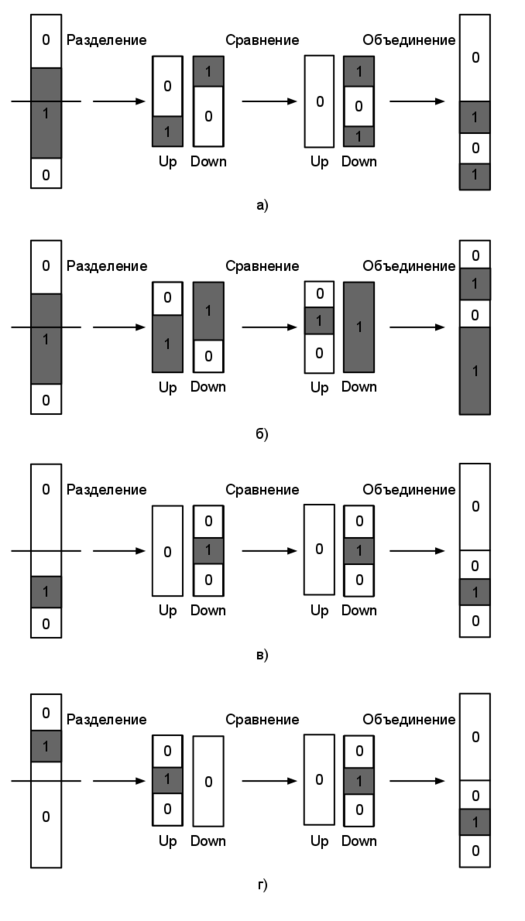
\includegraphics[scale=0.5]{snet2.png}\end{center}
Теперь используем полуфильтры для сортировки битонических последовательностей. Как только что было доказано, один полуфильтр разделяет битоническую последовательность на две равные части, одна из которых однородна, а другая сама по себе является битонической последовательностью, причем части расположены в правильном порядке. Тогда мы можем каждую часть снова отправить в полуфильтр вдвое меньшего размера, чем предыдущий. Затем, если нужно, четыре получившихся части снова отправить в полуфильтры и так далее, пока количество проводов в одной части больше 1.\\
 Поскольку каждый вертикальный ряд полуфильтров вдвое сокращает число входов, которые необходимо отсортировать, глубина всей сети равна $log_2n$, где n — число входов. Количество компараторов равно $\frac{n(log_2n)}{2}$, потому что в одном слое $\frac{n}{2}$ компараторов\\
\textbf{Объединяющая сеть} - сеть компараторов, объединяющая две отсортированные входные последовательности в одну отсортированную выходную последовательность.\\
Отсортированная последовательность имеет вид 0..01..1. Запишем две входные последовательности. Если перевернуть вторую последовательность, получится отсортированная по невозрастанию последовательность 1..10..0. Если теперь записать первую и перевернутую вторую последовательности подряд, получится битоническая последовательность, которую можно отсортировать в битоническом сортировщике с глубиной O(logn).\\
Объединяющая сеть является ничем иным как битоническим сортировщиком. Единственное отличие в том, что половина входных проводов расположена в обратном порядке (предполагается, что мы объединяем две сети одинакового размера $\frac{n}{2}$). Поэтому первый полуфильтр будет отличаться от остальных — он будет соединять i-ый провод не с $\frac{n}{2}$+i-ым, а с n-i+1-ым проводом. Схема объединяющей сети для восьми проводов приведена ниже.
\begin{center}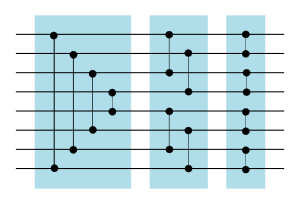
\includegraphics[scale=0.5]{snet3.png}\end{center}
Глубина и число компараторов в объединяющей сети очевидно те же, что и в битоническом сортировщике.\\
\textbf{Теперь, с помощью описанных выше объединяющих сетей мы построим параллельную версию сортировки слиянием.}
Чтобы отсортировать всю последовательность, мы сначала отсортируем пары, потом четверки, потом восьмерки и т.д. входных проводов.\\
\paragraph{Размер и глубина}(it's so deep)\\
Сеть состоит из $log_2n$ "слоев" объединяющих сетей. Такая сеть из слоя с номером i имеет глубину $log_2 2^i = i$, потому что объединяет $2^i$ проводов. Тогда глубина всей сети $\sum_{i=1}^{log_2n}{i}=\frac{(1+log_2n)log_2n}{2} = O(log^2n)$\\
Размер: в каждом слое сети $\frac{n}{2}$ компараторов => во всей сети $O(nlog^2n)$

\section{Деревья}
\subsection{Некоторые определения}
\begin{description}
	\item[дерево] - связный граф без циклов
	\item[корневой узел] - узел, не имеющий предков
	\item[лист] - узел, не имеющий потомков
	\item[внутренний узел] - узел, имеющий потомков
\end{description}
\subsection{Обход дерева}
\paragraph{Обход в глубину} Для обхода в глубину удобно использовать стек, в который по очереди в зависимости от порядка обхода кладется вершина, ее левый и правый ребенок. 
\paragraph{pre-order(прямой обход)}
\begin{enumerate}
	\item  Проверяем текущий узел на NULL
	\item  Выводим значение в текущем узле
	\item  Обходим прямым обходом левое поддерево
	\item  Обходим прямым обходом правое поддерево
\end{enumerate}

\paragraph{in-order(центрированный обход)}
\begin{enumerate}
	\item  Проверяем текущий узел на NULL
	\item  Обходим центрированным обходом левое поддерево
	\item  Выводим значение в текущем узле
	\item  Обходим центрированным обходом правое поддерево
\end{enumerate}

\paragraph{post-order(обратный обход)}
\begin{enumerate}
	\item  Проверяем текущий узел на NULL
	\item  Обходим обратным обходом левое поддерево
	\item  Обходим обратным обходом правое поддерево
	\item  Выводим значение в текущем узле
\end{enumerate}

\paragraph{Обход в ширину} - значения в вершинах выводятся по уровням слева направо\\
Для осуществления такого обхода надо завести очередь и положить в нее корень дерева. Пока очередь непуста, достаем из нее элемет, выводим его значение и кладем в очередь его левого и правого ребенка.
\subsection{Двоичное дерево поиска}
У каждой вершины не более 2х потомков, любое поддерево так же является деревом поиска, все ключи в левом поддереве меньше, чем в корне, в правом поддереве - больше, чем в корне. 
\paragraph{Поиск} - по ключу возвращаем ссылку на узел с таким же ключом\\
\textbf{Алгоритм} \\
\begin{itemize}
	\item Если текущий узел пуст - вернуть NULL
	\item Если ключ текущего узла равен искомому - вернуть ссылку на текущий узел 
	\item Если ключ текущего больше искомого - уйти в левое поддерево, иначе - в правое
\end{itemize}
\paragraph{Вставка} - рассматриваем случай, когда все ключи различны\\
\textbf{Алгоритм}\\
\begin{itemize}
	\item Если дерево пусто - заменить корень на узел с ключом равным данному, завершить работу
	\item Если ключ текущего больше искомого - уйти в левое поддерево, иначе - в правое
\end{itemize}
\paragraph{Удаление}
\textbf{Алгоритм}
\begin{itemize}
	\item Если текущий узел пуст - завершить работу
	\item Если ключ текущего больше данного - рекурсивно удалить ключ из левого поддерева, иначе - из правого
	\item Если ключ текущего узла равен искомому - рассмотреть случаи 
	\begin{enumerate}
		\item текущий узел - лист - удалили и не паримся
		\item у текущего узла один ребенок - поставили ребенка вместо текущего узла, текущий удалили
		\item у текущего узла два ребенка - возьмем m самый левый узел правого поддерева, удалим его из правого поддерева, поставим вместо текущего ключа ключ m
	\end{enumerate}
\end{itemize}
\subsection{Декартово дерево}
Курево(куча + дерево) - бинарное дерево, в узлах которого хранятся пары (ключ, приоритет). По ключам курево является двоичным деревом поиска, а по приоритетам - кучей.
\paragraph{split} - по дереву Т и ключу к split возвращает 2 дерева Т1 и Т2. В Т1 все ключи меньше к, в Т2 все ключи больше или равны к.\\
\textbf{Псевдокод}\\
\begin{center}
		\begin{lstlisting}
			<Treap*, Treap*> split(Treap* t, Key k){
				if(t == NULL) return <NULL, NULL>;
				if(t->key > k){
					<t1, t2> = split(t->left, k);
					t->left = t2;
					return <t1, t>;
				}else{
					<t1, t2> = split(t->right, k);
					t->right = t1;
					return <t, t2>;
				}
			}
		\end{lstlisting}
	\end{center}
Время работы алгоритма - О(h), где h - высота дерева, т.к. split рекурсивно проходит по вершинам в глубину дерева и на каждом шаге работает О(1)
\paragraph{merge} - по двум куревам Т1 и Т2, любой ключ в Т1 меньше любого ключа в Т2, merge строит курево Т, в котором есть все ключи из первого и второго дерева.\\
\textbf{Псевдокод}\\
\begin{center}
		\begin{lstlisting}
			Treap* merge(Treap* t1, Treap* t2){
				if(t1 == NULL) return t2;
				if(t2 == NULL) return t1;
				if(t1->priority > t2->priority){
					t1->right = merge(t1->right, t2);
					return t1;
				}else{
					t2->left = merge(t1, t2->left);
					return t2;
				}
			}
		\end{lstlisting}
	\end{center}
Время работы алгоритма - О(h), где h - высота дерева, т.к. split рекурсивно проходит по вершинам в глубину дерева и на каждом шаге работает О(1)
\paragraph{Вставка узла} split - merge - merge
split по ключу вставляемого узла\\
merge первого курева из возвращенной пары и вставляемого узла\\
merge этой штуки  с оставшимся куревом
\paragraph{Удаление по ключу} split - merge
split по ключу удаляемого узла\\
из второго курева из возвращенной пары удалим самого левого ребенка\\
merge этой штуки  с оставшимся куревом
\paragraph{Построение} - наивно - просто добавлять по порядку, каждая вставка за  О(log n), значит общая сложность  О(n log n)\\

\textbf{Алгоритм за O(n)} - если пары отсортированны по ключу по возрастанию\\
Будем строить дерево слева направо, то есть начиная с (x1,y1) по (xn,yn), при этом помнить последний добавленный элемент (xk,yk). Он будет самым правым, так как у него будет максимальный ключ, а по ключам декартово дерево представляет собой двоичное дерево поиска. При добавлении (xk+1,yk+1), пытаемся сделать его правым сыном (xk,yk), это следует сделать если yk>yk+1, иначе делаем шаг к предку последнего элемента и смотрим его значение y. Поднимаемся до тех пор, пока приоритет в рассматриваемом элементе меньше приоритета в добавляемом, после чего делаем (xk+1,yk+1) его правым сыном, а предыдущего правого сына делаем левым сыном (xk+1,yk+1).\\
Заметим, что каждую вершину мы посетим максимум дважды: при непосредственном добавлении и, поднимаясь вверх (ведь после этого вершина будет лежать в чьём-то левом поддереве, а мы поднимаемся только по правому). Из этого следует, что построение происходит за O(n).
\paragraph{Теорема про случайные приоритеты} по сути про то, что глубина О(n log n)\\
coming soon...\\

\subsection{АВЛ - дерево}

	\paragraph{Основное свойство} - сбалансированность \\
	Для каждой вершины $|h(l) - h(r)| \leq 1$, где $h(l)$ - глубина левого поддерева, $h(r)$ - глубина правого поддерева \\
	
	\paragraph{Высота} $O(\log N)$ \\
	\textbf{Доказательство} - по индукции докажем, что минимальное число вершин в AVL-дереве высоты $h$: $m_{h} = F_{h+2} - 1$, где $F_{h}$ - $h$-ое число Фибоначчи. \\
	$m_{h+2}$ = $m_{h+1} + m_{h} + 1$, т.к. разница между высотой детей не больше 1. \\
	Далее доказательство по индукции.\\
	$F_{h} = \Omega(\phi^{h})$, где $\phi$ - константа. \\
	Получаем $n \geq \phi^{h} \Leftrightarrow \log_{\phi} n \geq h$ \\
	
	\textbf{Как балансировать дерево?} - очень просто \\
	Поворот производим, если разница высот равна 2. \\
	Существует два основных типа поворота - правый и левый, но не всегда мы можем сразу выполнить поворот. \\
	Мы можем сделать левый поворот, если высота правого ребёнка больше левого и \textbf{высота правого ребёнка правого ребёнка (т.е. самого правого внука изначальной вершины) больше или равна высоте левого ребёнка правого ребёнка} \\
	Правый поворот при аналогичных условиях, т.е. высота левого ребёнка больше правого и \textbf{высота левого ребёнка левого рёбнка (т.е. самого левого внука изначальной вершины) больше или равна высоте правого ребёнка левого ребёнка} \\
	\textbf{Как выполняется поворот?} - разберём на примере левого поворота, для правого аналогично \\
	Мы "поднимаем" правого ребёнка наверх, при этом он неожиданно становится родителям троих детей, так у нас не принято, поэтому одного ребёнка нужно отдать другому ребёнку, отличный кандидат для этого - предыдущий левый ребёнок правого ребёнка, т.к. неожиданно у нашей рассматриваемой ноды (для которой мы осуществляли поворот) остался только один ребёнок. \\
	
	\textbf{Звучит сложно?} Тогда посмотрим картинки. \\
	
	\begin{center}
	\textbf{Выполняем левый поворот. Случай, когда правый ребёнок правого ребёнка больше.} \\
	\begin{forest}
		for tree={
			grow=south,
			circle, draw, minimum size=3ex, inner sep=1pt,
			s sep=7mm
			}
		[5
			[3
			]
			[10
				[7
				]
				[15
					[12
					]
					[20
					]
				]
			]
		]
	\end{forest} \\
	
	\textbf{Дерево переходит в следующий вид} \\
	
	\begin{forest}
		for tree={
			grow=south,
			circle, draw, minimum size=3ex, inner sep=1pt,
			s sep=7mm
			}
		[10
			[5
				[3
				]
				[7
				]
			]
			[15
				[12
				]
				[20
				]
			]
		]
	\end{forest}
	\end{center}
	
	Если же мы не можем сразу сделать поворот, но баланс нарушен, то нужно спуститься к ребёнку (правому, если у нас левый поворот, иначе левому) и сделать поворот в другую сторону уже относительно него, чтобы привести дерево в подходящий вид. \\
	\textbf{Посмотрим картинки} 
	\begin{center}
	\textbf{Выполняем левый поворот. Случай, когда левый ребёнок правого ребёнка больше, поэтому сначала делаем правый поворот для правого ребёнка} \\
	\begin{forest}
		for tree={
			grow=south,
			circle, draw, minimum size=3ex, inner sep=1pt,
			s sep=7mm
			}
		[5
			[3
			]
			[10
				[7
					[6
					]
					[8
					]
				]
				[15
				]
			]
		]
	\end{forest} \\
	\textbf{Для начала сделаем правый поворот для правого ребёнка} \\
	\begin{forest}
		for tree={
			grow=south,
			circle, draw, minimum size=3ex, inner sep=1pt,
			s sep=7mm
			}
		[5
			[3
			]
			[7
				[6
				]
				[10
					[8
					]
					[15
					]
				]
			]
		]
	\end{forest} \\
	\textbf{Теперь можем спокойно сделать левый поворот} \\
	\begin{forest}
		for tree={
			grow=south,
			circle, draw, minimum size=3ex, inner sep=1pt,
			s sep=7mm
			}
		[7
			[5
				[3
				]
				[6
				]
			]
			[10
				[8
				]
				[15
				]
			]
		]
	\end{forest} \\
	\end{center}
	
	\paragraph{Операции} - вставка \\
	Ищем место для вставки как в обычном бинарном дереве, вставляем, далее запускаем балансировку от места вставки \\
	\textbf{Удаление} \\
	Ищем элемент для удаления как в обычном бинарном дереве, далее 3 случая:
	\begin{itemize}
		\item Вершина без детей - тупо вырезаем, обнуляем указатели родителя на неё
		\item Вершина с ребёнком - вырезаем, подцепляем ребёнка с родителю
		\item Вершина с двумя детьми - находим ближайшую вершину для удаляемой (например, самую правую в левом поддереве), меняем значения, запускаем удаление от найденной вершины
	\end{itemize}

\subsection{Красно-черное дерево}
 двоичное дерево поиска, в котором баланс осуществляется на основе "цвета" узла дерева, который принимает только два значения: "красный" и "чёрный"\\
При этом все листья дерева являются фиктивными и не содержат данных, но относятся к дереву и являются чёрными. "Объединим" их в один NIL\\
\paragraph{Свойства}
\begin{enumerate}
	\item Каждый узел промаркирован красным или чёрным цветом
	\item Корень и конечные узлы (листья) дерева — чёрные
	\item У красного узла родительский узел — чёрный
	\item Все простые пути из любого узла x до листьев содержат одинаковое количество чёрных узлов
	\item Чёрный узел может иметь чёрного родителя
\end{enumerate}
\paragraph{Высота красночерного дерева} - определение
Черная высота вершины x - число чёрных вершин на пути из x в лист.\\
\textbf{Лемма} В красно-черном дереве высотой $hb$ количество внутренних вершин не менее $2^{hb-1}-1$\\
доказывается по индукции по высоте дерева\\
\textbf{Теорема} Красно-черное дерево с n ключами имеет высоту О(log n)\\
Рассмотрим красно-чёрное дерево с высотой $h$. Так как у красной вершины чёрные дети (по свойству 3) количество красных вершин не больше $\frac{h}{2}$. Тогда чёрных вершин не меньше, чем $\frac{h}{2} - 1$\\
По лемме для дерева размера n\\
$n \geq 2^{\frac{h}{2}}-1$\\
Прологарифмировав неравенство, имеем:\\
$h \geq 2log(n+1)$\\
\paragraph{Вставка}
Вставка узла производится на меcто NIL'а. Вставляем вершину вместо NIL с нулевыми потомками и красим в красный цвет. \\
\begin{center} Балансировка для вершины х \end{center}
\begin{description}
	\item[]Отец - черный - все ок
	\item[]Отец - красный - нарушается свойство 3 (при этом отец точно не корень, значит есть и дедушка)\\
\begin{enumerate}
	\item Дядя - красный\\
		Перекрасим отца и дядю в черный, деда в крассный. Поддерево с вершиной х - сбалансированно. Теперь балансируем деда.\\
\begin{center}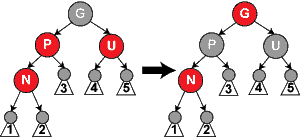
\includegraphics{rbt_in_ru.png}\end{center} 

	\item Дядя - черный\\
Пусть о - отец, д - дед, т - дядя вершины х\\
		Рассмотрим случай, когда о - левый ребенок д. Правый симметрично\\
		Если х - правый ребенок о, выпоним левый поворот: о становится левым ребенком х, х становится на место о.\\
		Теперь можем совершить правый поворот, т.е. корнем поддерева станет левый ребенок д, д станет правым ребенком нового корня. Т.к. до вставки х дерево было сбалансированно, д - черная вершина. Перекрасим д в красный, новый корень в черный. Свойства сохранятся\\
\begin{center}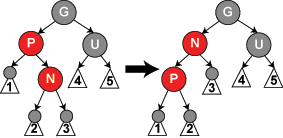
\includegraphics{rbt_in_bu.png}\end{center} 
\end{enumerate}
\end{description}
\paragraph{Удаление}(видимо тебя из этой жизни)\\
\begin{center} Удаление в зависимости от количества детей \end{center}
\begin{enumerate}
	\item Если у вершины нет ненулевых детей, то баланируем и изменяем указатель на неё у родителя на NIL
	\item Если у неё только один ненулевой ребёнок, то балансируем и делаем у родителя ссылку на него вместо этой вершины.
	\item Иначе находим наименьший элемент в правом поддереве(сначала мы переходим в правое поддерево, а после спускаемся вниз в левое до тех пор, пока у вершины есть левый ненулевой ребенок), копируем его значение в удаляемый, удаляем его рекурсивно из правого поддерева по 1му или 2му пункту.
\end{enumerate}
Заметим, что балансировать удаляемую вершину, у которой 2 ребенка не надо, т. к. в ней ничего не изменилось, кроме значения, а значит свойства могли сломаться только у наименьшего элемента в правом поддереве, который мы удалили.
А дальше - балансировка!\\
Если вершина была красной, то и балансировать даже не надо.
Если она была черной, то если ее ребенок был красным, просто перекрасим его в черный.\\
Иначе и удаляемая вершина и ее ребенок - черные.\\
Дальше рассматриваем случай, когда n - левый ребенок. Правый симметрично.
Итак, удалили вершину n, на ее месте теперь ребенок n и он черный(назовем его х). Исходим из того, что брат х - черный.\\
Если брат х - красный, то совершим левый поворот вокруг нового родителя х, перекрасим родителя в красный, а брата в черный. Сейчас брат стал дедушкой х. Т.к. он был красный, его дети черные, его левый ребенок стал братом х, значит у х сейчас черный брат.\\
\begin{center}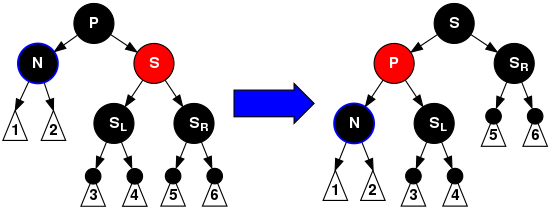
\includegraphics[scale=0.7]{rbt_del_1.png}\end{center} 
Теперь рассмотрим случаи:
\begin{enumerate}
	\item Если оба ребенка брата - черные, перекрасим брата в красный. Тогда поддерево с корнем в родителе х сбалансированно. При этом, если родитель х был красным, перекрасим его в черный и дерево окажется сбалансированным, иначе все пути, идущие через родителя х, имеют черную глубину на один меньше, чем все остальные. Тогда запустим балансировку от родителя\\
\begin{center}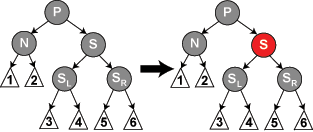
\includegraphics{rbt_del_2.png}\end{center}
	\item Если левый ребенок брата - красный, а правый - черный, то совершим правый поворот вокруг брата. Его красный ребенок станет новым отцом. Поменяем цвета нового отца и брата. у х теперь есть черный брат с черным левым и красным правым потомком. Переходим к следующему случаю.\\
\begin{center}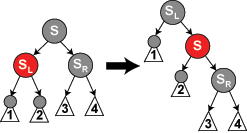
\includegraphics{rbt_del_4.png}\end{center}
	\item Левый ребенок брата - черный, а правый - красный. Совершим поворот относительно отца х влево. Поменяем цвета отца и брата местами, т.е. отец станет черным, а черная высота левого поддерева брата(нового отца) увеличится на 1, а правого уменьшится на 1. Перекрасим правого ребенка брата в черный\\
\begin{center}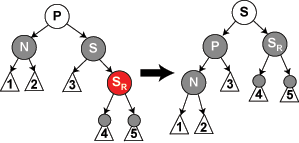
\includegraphics{rbt_del_5.png}\end{center}
\end{enumerate}
\paragraph{Оценка сложности} - прямо с wiki, так что придется подкорректировать \\
Все рекурсивные вызовы функции хвостовые и преобразуются в циклы, так что алгоритм требует памяти O(1). В алгоритме выше, все случаи связаны по очереди, кроме случая 3, где может произойти возврат к случаю 1, который применяется к предку узла: это единственный случай когда последовательная реализация будет эффективным циклом (после одного вращения в случае 3).

Так же, хвостовая рекурсия никогда не происходит на дочерних узлах, поэтому цикл хвостовой рекурсии может двигаться только от дочерних узлов к их последовательным родителям. Произойдет не более, чем O(log n) циклических возвратов к случаю 1 (где n — общее количество узлов в дереве до удаления). Если в случае 2 произойдет вращение (единственно возможное в цикле случаев 1-3), тогда отец узла N становится красным после вращения и мы выходим из цикла. Таким образом будет произведено не более одного вращения в течение этого цикла. После выхода из цикла произойдет не более двух дополнительных поворотов. А в целом произойдет не более трех поворотов дерева. \\
\paragraph{Оценка сложности (альтернативная)} - \textbf{вставка} \\
Только при чёрном дяде мы выполняем балансировку для деда, таких переходов будет не больше $O(h)$, где $h$ -высота дерева, т.е. вставка за $O(\log n)$ \\
\textbf{Удаление} \\
Только в случае чёрного брата с чёрными детьми мы запускаем балансировку от родителя, таких переходов будет не больше $O(h)$, где $h$ -высота дерева, т.е. вставка за $O(\log n)$, в остальных случаях завершение происходит после выполнения фиксированного числа изменений цвета и не более трёх поворотов \\

\subsection{Сплей-дерево}
\paragraph{О что это?} - двочиное дерево поиска, которое обеспечивает быстрый доступ к данным, которые недавно использовались, дерево самобалансируется так, что поддерживает сложность $O(\log n)$ для всех операций (поиск, вставка, удаление), суть в том, что операции добавления и поиска отправляют использованную вершину в корень, но как? \\
\paragraph{Операция splay} - операция расширешия \\
Этой операцией мы отправляем вершину в корень с помощью комбинации трёх отдельных операций:
\begin{itemize}
	\item Zig - выполняем, если родитель вершины - корень, по сути, обычный левый/правый поворот соответственно в зависимости от того, каким ребёнком явлется наша вершина \\
	\textbf{Пример: до} \\
	\begin{center}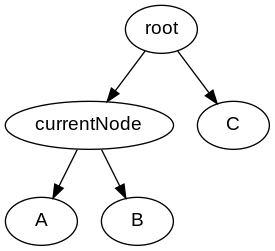
\includegraphics[scale=0.7]{splayZigBefore.png}\end{center} 
	\textbf{После} \\
	\begin{center}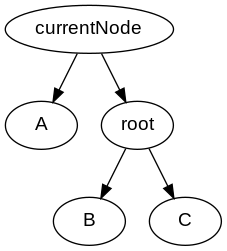
\includegraphics[scale=0.7]{splayZigAfter.png}\end{center} 
	\item Zig-Zig - два простых поворота, выполняются, если и текущая вершина, и её родитель являются одним и тем же типом ребёнка (например, оба левые, тогда сначала производим правый поворот относительно деда, потом относительно родителя) \\
	\textbf{Пример: до} \\
	\begin{center}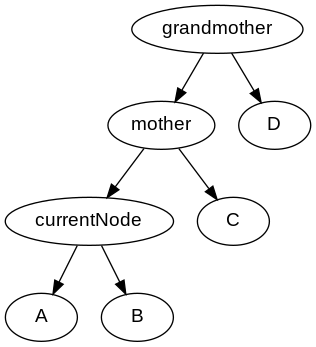
\includegraphics[scale=0.7]{splayZigZigBefore.png}\end{center} 
	\textbf{После} \\
	\begin{center}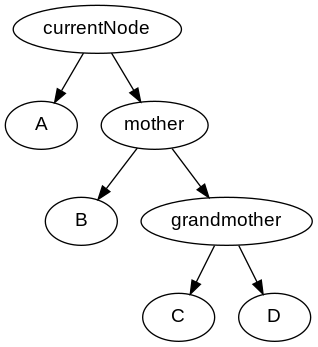
\includegraphics[scale=0.7]{splayZigZigAfter.png}\end{center} 
	\item Zig-Zag - большой левый или большой правый поворот, выполняется в тех же случаях, что и для AVL дерева \\
	\textbf{Пример: до} \\
	\begin{center}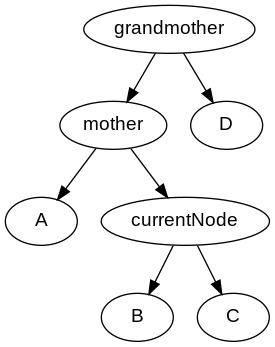
\includegraphics[scale=0.7]{splayZigZagBefore.png}\end{center} 
	\textbf{После} \\
	\begin{center}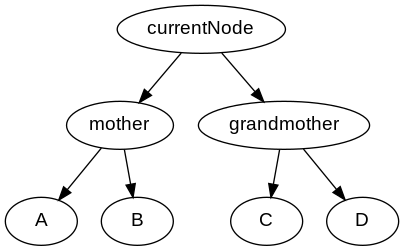
\includegraphics[scale=0.7]{splayZigZagAfter.png}\end{center} 
\end{itemize} 

\textbf{Основные операции} \\
\begin{itemize}
	\item Search - ищем как в бинарном дереве, потом запускаем splay от найденной вершины
	\item Split - находим ближайший элемент к ключу, делаем для него splay, отрезаем левого ребёнка и возвращаем его вместе с корнем
	\item Merge - находим самый правый элемент в первом дереве, делаем для него splay, подцепляем справа второе дерево
	\item Insert - делаем split по вставляемому ключу, потом подцепляем полученные деревья к новой вершине
	\item Delete - ищем элемент как в бинарном дереве, запускаем от него splay, возвращаем merge его детей
\end{itemize}

\subsection{B - деревья}
B-дерево - сбалансированное сильно ветвящееся дерево поиска. В каждом узле хранятся массивы ключей. t - параметр дерева.
\paragraph{Применение}
Структура B-дерева применяется для организации индексов во многих современных СУБД.\\

B-дерево может применяться для структурирования (индексирования) информации на жёстком диске (как правило, метаданных). Время доступа к произвольному блоку на жёстком диске очень велико (порядка миллисекунд), поскольку оно определяется скоростью вращения диска и перемещения головок. Поэтому важно уменьшить количество узлов, просматриваемых при каждой операции. Использование поиска по списку каждый раз для нахождения случайного блока могло бы привести к чрезмерному количеству обращений к диску вследствие необходимости последовательного прохода по всем его элементам, предшествующим заданному, тогда как поиск в B-дереве, благодаря свойствам сбалансированности и высокой ветвистости, позволяет значительно сократить количество таких операций.\\

Относительно простая реализация алгоритмов и существование готовых библиотек (в том числе для C) для работы со структурой B-дерева обеспечивают популярность применения такой организации памяти в самых разнообразных программах, работающих с большими объёмами данных.\\
\paragraph{Принцип построения}
\begin{enumerate}
	\item Ключи в узле упорядочены.
	\item Корень содержит от 1 до 2t-1 ключей.
	\item Любой другой узел содержит от t-1 до 2t-1 ключей.
	\item Любой узел кроме листа, содержащий n: $k_1, k_2, ..., k_n$ ключей, содержит n потомков. При этом:
\begin{itemize}
	\item Первый потомок содержит ключи меньшие $k_1$
	\item Для $2 \leq i \leq n$ i-й потомок содержит ключи из инетрвала ($k_{i-1}, k_i$)
	\item Последний потомок содержит ключи большие $k_n$
\end{itemize}
	\item Глубина всех листьев одинакова.
\end{enumerate}
\paragraph{Поиск} Если ключ содержится в данной вершине, он найден, иначе переходим к интервалу между двумя ключами данной вершины, в которой лежит искомый ключ и идем к соответствующему потомку.
\paragraph{Вставка}
Ищем лист, в который можно добавить ключ. Если в найденном листе меньше 2t-1 ключей, добавляем в него наш ключ.\\
Иначе после добавления нашего ключа в листе оказывается 2t ключей. Теперь разбиваем узел на 2 узла - первые t ключей и последние t-1 ключей. Оставшийся средний элемент вставлям в родительский узел между ключами, между которыми находился найденный лист.\\
Если родительский узел заполнен, повторяем разделение, пока не найдем незаполненный узел или не дойдем до корня.\\
Если дошли до корня, то разобьем его на 2 узла, а средний ключ корня сделаем новым корнем.\\
\paragraph{Удаление}
Ищем узел, в котором находится удаляемый ключ. Возможны два случая:\\
\textbf{Удаление из листа}\\
Если в узле больше t-1 ключей, просто удаляем наш.\\
Иначе, если найдется соседний лист с тем же родителем, в котором больше t-1 ключей, выберем из соседа ближайший к нашему листу ключ, поместим его в "разделяющий" элемент родителя, а этот элемент спустим в наш лист. Удалим из листа нужный ключ.\\
Если соседей - буржуев не оказалось, то листы - пролетарии соединяются...  Объединяем наш лист и одного из его соседей, удаляем наш ключ, перемещаем разделяющий ключ из родителя в новый лист.\\
\textbf{Удаление из внутреннего узла}\\
Если левый(правый) дочерний узел для ключа, который мы хотим удалить, содержит более t-1 ключей, перемещаем из него крайний правый(левый) ключ на место удаляемого.\\
Иначе в обоих дочерних узлах t-1 ключей. Тогда соединяем их, а удаляемый ключ, просто удаляем, располагая указаатель на новый узел там, где был этот ключ.\\
Если сливаются 2 последних потомка корня – то они становятся корнем, а предыдущий корень освобождается.\\ 
\subsection{Алгоритм Хаффмана}
\paragraph{Определение} - алгоритм оптимального префиксного кодирования алфавита. Пусть $A = {a_1,.., a_n}$ - алфавит из $n$ различных символов, $W = {w_1,.., w_n}$ - набор весов. Тогда бинарный набор кодов $C = {c_1,.., c_n}$, где $c_i$ - код символа $a_i$, такой, что:
\begin{itemize}
	\item $c_i$ не является префиксом другого кода 
	\item сумма произведений длинн кодов на их частоту минимальна
\end{itemize}
\paragraph{Построение дерева кодирования} за $O(n)$
\begin{itemize}
	\item Сортируем массив частот
	\item Создаём второй массив, заполненный бесконечностями
	\item Заводим указатели на начало
	\item Добавляем во второй массив сумму двух минимальных элементов среди 4 элементов (первые 2 элемента первого массива и первые 2 элемента второго)
	\item Сдвигаем указатели
\end{itemize}
\textbf{Теорема об оптимальности префиксного кода алгоритма Хаффмана} \\
\textbf{Лемма 1. Докажем, что для алфавита существует оптимальный префиксный код, в котором два символа с самыми низкими частотами имеют одинаковую длину и отличаются лишь последним битом} \\
Докажем возможность преобразовать дерево с произвольным оптимальным префиксным кодом в другое дерево с оптимальным префиксным кодов, в котором данные символы ($x$ и $y$ являются листьями с общим родителем, причем они находятся на максимальной глубине \\
Пусть $a$ и $b$ - листья с общим родителем на максимальной глубине в оптимальном дереве $T$. Пусть $a.freq \leq b.freq$ и $x.freq \leq y.freq$. Будем считать, что $x \neq b$. \\
Пусть мы получили дерево $T'$ перестановкой $a$ и $x$ и дерево $T''$ перестановкой $b$ и $y$ \\
Тогда разность стоимостей $T$ и $T'$ равна:
\[
	B(T) - B(T') = \sum_{c \in C} c.freq*h_T (c) - \sum_{c \in C} c.freq*h_{T'} (c) = x.freq * h_T(x) + a.freq * h_T(a) - x.freq * d_{T'}(x) - a.freq * d_{T'}(a) = x.freq * h_T(x) + a.freq * h_T(a) - x.freq * h_T(a) - a.freq * h_T(x) = (a.freq - x.freq)(d_T(a) - d_T(x)) \geq 0
\]
Аналогично второй обмен не увеличивает стоимости, т.е. $B(T') - B(T'') \Leftrightarrow B(T'') \leq B(T) $, но $T$ - оптимальное дерево $\Leftrightarrow B(T) \leq B(T'') \Leftrightarrow B(T'') = B(T)$, т.е. $T''$ - оптимальное дерево

Из \textbf{леммы 1} следует, что построение оптимального дерева путём объединения узлов можно начать с жадного выбора, при котором объединяются два символа с наименьшими частотами \\
Теперь докажем \textbf{лемму 2} про объединение узлов \\
Пусть у нас есть алфавит $C$, в котором символы $x, y$ - символы с минимальными частотами и алфавит $C'$, полученный из $C$ удалением символов $x,y$ и добавлением нового символа $z$ ($z.freq = x.freq + y.freq$). Пусть $T'$ - дерево оптимального префиксного кода для алфавита $C'$. Тогда дерево $T$, полученное из дерева $T'$ заменой листа $z$ внутренним узлом с детьми $x,y$, представляет оптимальный префиксный код для $C$ \\
Выразим $B(T)$ через $B(T')$\\
Для всех символов кроме $x, y$ из $C$ высота $h$ не изменилась, учитывая $h_T(x) = h_T(y) = h_{T'}(z) + 1$:
\[
	x.freq * h_T(x) + y.freq * h_T(y) = (x.freq + y.freq)(h_{T'}(z) + 1) = z.freq*h_{T'}(z) + (x.freq + y.freq)
\]
\[
	B(T) = B(T') + x.freq + y.freq \Leftrightarrow B(T') = B(T) - x.freq - y.freq
\]

Пусть дерево $T$ не является деревом оптимального префиксного кода, тогда $\exists T'' \colon B(T'') < B(T)$ \\
При чём из \textbf{леммы 1} мы получаем, что $x,y$ можно считать детьми одного и того же узла $T''$ \\
Рассмотрим дерево $T'''$, которое получено из дерева $T''$ заменой родителя $x,y$ на лист $z$ с частотой $z.freq = x.freq + y.freq$:
\[
	B(T''') = B(T'') - x.freq - y.freq < B(T) - x.freq - y.freq = B(T')
\]
Противерочие, т.к. $T'$ - дерево оптимального кода для $C'$ \\
Из \textbf{лемм 1 и 2} следует, что алгоритм построения дерева Хаффмана с жадным выбором позволяет получить оптимальное дерево
 
\section{Просто 4й модуль}
\subsection{Хеш - таблицы}
Хеш-таблица - структура данных, позволяющая выполнять операции поиска, вставки и удаления элемента в среднем за О(1) (реализующая интерфейс ассоциативного массива).\\
\textbf{Общая схема работы}\\
\begin{enumerate}
	\item По ключу вычисляется хеш-функция (возващает ключ - номер элемента в массиве)
	\item По номеру пытаемся сделать операцию, если произошла коллизия(ячейка уже занята) - разрешаем ее
\end{enumerate}
\paragraph{Хеш - функция} - превратит входной ключ в фарш.\\
Хеш-функция ― преобразование по детерминированному алгоритму входного массива данных произвольной длины (один ключ) в выходную битовую строку фиксированной длины (значение). Результат вычисления хеш-фукнции называют «хешем».\\
\textbf{Виды хеш-функций}(М - размер массива)
\begin{enumerate}
	\item Деление с остатком\\
Хеш-функция может вычислять «хеш» как остаток от деления входных данных на М.\\
При этом не следует использовать в качестве М степень основания системы счисления компьютера, т.к. хеш в таком случае будет зависеть только от нескольких последний битов входных данных, что приведет к большому количеству коллизий. Рекомендуется выбирать простое М.
	\item Мультипликативная схема хешировнаия\\
$h(k) = [M \cdot \{ k \cdot A \} ] $, где $0 < A < 1$\\
Кнут предложил выбирать в качестве А число как можно ближе к $\phi^{-1} = \frac{\sqrt{5} - 1}{2}$\\
Пусть $M = 2^{p}$, а $\omega = 2^{32}$ - длина машинного слова ($M < \omega$).\\
Возьмем $A = \frac{2654435769}{\omega}$\\ 
$h(k) = [2^{p} \cdot \{\frac{r_1 \cdot 2^{32} + r_0}{2^{32}}\}] = [2^p\cdot \frac{r_0}{2^{32}}] = [\frac{r_0}{2^{32-p}}]$\\
Таким образом хеш-функция вернет первые р бит $r_0$\\
$h(k) = (k\cdot s$ mod $2^{32}) >> (32 - p)$
	\item Полиномиальное хеширование\\
Пусть входные данные можно представить как $\{k_0, k_1, ..., k_n \}$ - некоторые числа. Тогда поделим с остатком многочлен $K(x) = k_0 + k_1x + ... + k_n x^n$ на заранее определенный для хеш-функции порождающий многочлен $P(x) = p_0 + ... + p_m x^m$\\
Тогда пусть хеш-функция возвращает коэфициенты многочлена, полученного при делении К на Р с остатком.
	\item Хеш для строки\\
Если есть строка $s = s_0, s_1, ..., s_n$, то определим хеш-функцию $h(s) = (s_0a^n + s_1a^{n-1} + ... + s_n)$ mod M\\
Если выбрать а и М взаимно простыми, то при изменении любого символа строки изменится и хеш(доказывается изходя из того, что для взаимно простыъ а и М $\{s\cdot a$ mod $M$ | $ 0\leq s < M\}=\{0, 1, ..., M-1\}$ )\\
Чтобы сократить количество операций сложения и умножения используют схему Горнера, т.е. представляют $h(k) = (((s-0a + s_1)a+s_2)a+ ... + s_{n-1})a+s_n$
\end{enumerate}

\paragraph{Разрешение коллизий методом цепочек}
Хеш-таблица представлена массивом, ячейка i которого хранит указатель на начало списка всех элементов, хеш-код которых равен i.\\
Если мы хотим найти элемент, вычисляем хеш и проходим по списку в ячейке с номером, равным хешу. Хотим вствить/удалить - вставляем/удаляем в список.\\
Соответственно, время работы поиска в худшем случае О(n), в среднем О(1)\\
\paragraph{Разрешение коллизий методом прямой адресации}
Все элементы непосредственно хранятся в массиве. При таком подходе таблица может оказаться полностью заполненна, поэтому возникнет необходимость увеличивать размер таблицы и перехешировать уже имеющиеся элементы. В реальности, т.к. по мере роста заполненности таблицы вероятность коллизии резко возрастает, расширение таблийы производят не при полном заполнении, а при заполненности $\frac{n}{m} > \alpha$, где $\alpha$ - заданное число меньше 1.\\
При поиске(удалении)элемента вычисляем его хеш, переходим в нужную ячейку и если она не содержит нужный элемент делаем последовательность проб - вычисляем новые номера ячеек, где мог бы находиться нужный элемент. Пока мы не находим нужный ил иячейка не оказвается пуста продолжаем, после выводим результат поиска.\\
При вставке пробы делаем, пока ячейка, куда мы хотим вставить элемент не пуста.\\
При этом может оказаться, что мы удалили элемент, а потом хотим найти элемент с таким же хешем, который был добавлен позже, т.е. лежит дальше ("через несколько проб"). В таком случае нам нужно, чтобы при поиске и удалении мы не останавливались на ячейках, где лежали удаленные элементы, а при вставке нам не важно было ли раньше что-то в той ячейке, куда мы хотим вставить, поэтому для ячеек мы заводим метку deleted, чтобы понимать, было ли удалено что-то из данной ячейки.\\
\subparagraph{Последовательности проб}
Пробирование - вычисление последовательности индексов, по которым располагаются элементы с определенным хешем.
\begin{enumerate}
	\item \textbf{Линейное пробрование}\\
 ячейки хеш-таблицы последовательно просматриваются с некоторым фиксированным интервалом k между ячейками (обычно k = 1), то есть i-й элемент последовательности проб — это ячейка с номером (hash(x) + ik) mod N. Для того, чтобы все ячейки оказались просмотренными по одному разу, необходимо, чтобы k было взаимно-простым с размером хеш-таблицы.
	\item \textbf{Квадратичное пробрование}\\
интервал между ячейками с каждым шагом увеличивается на константу. Если размер хеш-таблицы равен степени двойки (N = 2p), то одним из примеров последовательности, при которой каждый элемент будет просмотрен по одному разу, является:
hash(x) mod N, (hash(x) + 1*1) mod N, (hash(x) + 2*2) mod N, (hash(x) + 3*3) mod N, …
	\item \textbf{Двойное хеширование}\\
интервал между ячейками фиксирован, как при линейном пробировании, но, в отличие от него, размер интервала вычисляется второй, вспомогательной хеш-функцией, а значит, может быть различным для разных ключей. Значения этой хеш-функции должны быть ненулевыми и взаимно-простыми с размером хеш-таблицы, что проще всего достичь, взяв простое число в качестве размера, и потребовав, чтобы вспомогательная хеш-функция принимала значения от 1 до N — 1.
\end{enumerate}
\subparagraph{Проблема кластеризации}
При использовании первых двух способов пробирования часто возникают кластеры.\\
Кластер - последовательность занятых ячеек. В ячейку кластера может попасть элемент с любым хешем на некоторой пробе. При образовании такой последовательности следующий попадающий в ячейку кластера элемент в итоге проходит по ячейкам кластера и увеличивает его, тогда операции над хеш таблицей начинают выполняться за линейное время.
\section{Жадные алгоритмы, ДП}
\subsection{Общая идея жадных алгоритмов}
\paragraph{Идея} в том, что на каждом шагу алгоритма мы выбираем локально наилучший выбор в надежде, что итоговое решение будет оптимальным. Пример: Дейкстра, задача о раписании \\
Такой алгоритм применим к задачу, есои последовательность локально оптимальных выборов даёт глобально оптимальное решение и оптимальное решение задачи содержит в себе оптимальные решения для всех её подзадач \\
\subsection{Динамическое программирование, идея}
\paragraph{Общий принцип} - динамическое программирование обычно применяется к задачам оптимизации, когда среди множества возможных решений необходимо выбрать оптимальное. Идея в том, что оптимальное решение подзадач меньшего размера может быть использовано для решения исходной задачи. \\
\textbf{Основные свойства} \\
\begin{itemize}
	\item Задача разбивается на подзадачи
	\item Подзадачи \textbf{немного} меньше задачи
	\item Подзадачи решаются тем же методом
	\item Имеется процесс консолидации (т.е. для решения задачи используются решения подзадач)
	\item Имеется порядок на подзадачах (т.е. мы знаем, какие подзадачи решаем раньше, и нет такого, что в решении текущей задачи используется подзадача, для решения которой нужна текущая задача)
	\item Часть подзадач совпадает
\end{itemize}
Процесс разработки алгортма можно разделить на этапы:
\begin{itemize}
	\item Разбиение задачи на подзадачи меньшего размера
	\item Нахождение оптимального решения подзадач рекурсивно
	\item Использование полученного решения подзадач для конструирования решения исходной задачи
\end{itemize}
\paragraph{Нисходящее ДП} - обычная рекурсивная реализация, когда подзадача испольует в своём решении данные о решении следующей подзадачи, обычно такая реализация используется вместе с запоминанием (кэшированием) \\
\paragraph{Идея запоминания} - перед непосредственным вычислением функция проверяет, не была ли решена конкретная подзадача до этого \\
\paragraph{Восходящее ДП} - принцип построения решения так, что к моменту, когда мы непосредственно столкнёмся с задачей, все подзадачи будут решены \\
А теперь на конкретных задачах
\subsection{Вычисление числа Фибоначчи}
Легко решить с помощью восходящего ДП (также можно с помощью нисходящего с запоминанием) \\
\begin{center}
		\begin{lstlisting}
			size_t F[n];
			F[0] = 1;
			F[1] = 1;
			for(int i = 2; i < n; i++) {
				F[i] = F[i - 1] + F[i - 2];
			}
		\end{lstlisting}
\end{center}
\subsection{Задача о рюкзаке}
Пусть есть набор предметов ${n_1, n_2,...,n_k}$, где $n_i$ - стоимость $i$-ого предмета, $k$ - количество предметов из набора, которые мы берём, $s$ - вместимость рюкзака \\
Решается динамическим соотношением $A(k, s) = max(A(k-1, s), A(k-1,s-w_k) + p_k)$, где $w_k$ - вес $k$-ого предмета, $p_k$ - стоимость $k$-ого предмета \\
Восстановить решение можно от ответа, если сверять значение $A(i,w)$ с $A(i-1,w)$ и $A(i-1, w-w_i) + p_i$ \\
\subsection{Нахождение наибольшей возрастающей подпоследовательности}
\textbf{Решение за $O(n^2)$} \\
Построим массив $d$, где $d[i]$ - это длина наибольшей возврастающей подпоследовательности, которая оканчивается в элементе с индексом $i$, будем заполнять массив постепенно, тогда $d[i] = 1 + max_{j=0..(i-1)} d[j]$, при условии, что $a[j] < a[i]$, т.е. мы выбираем максимальную возврастающую подпоследовательность с учётом того, что подпоследовательности в некоторых случаях мы можем продлить \\
Чтобы получить саму последовательность индексов, нам нужно восстановить решение, для этого заведём вспомогательный массив $prev$: $prev[i] = $ индекс элемента в исходном массиве, при котором достигается $d[i]$ \\
\textbf{Решение за $O(n \log n)$} \\
Модифицируем массив $d$, пусть теперь $d[i]$ - наименьшее число, на которое оканчивается возрастающая последовательность длины $i$, тогда $\forall i d[i-1] \leq d[i]$, к тому же каждый элемент $a[i]$ обновляет максимум один элемент $d[j]$, тогда при обработке очередного $a[i]$ будем бин. поиском по $d$ искать первое число, которое больше или равно $a[i]$ и обновлять его (т.е. если $d[j-1] < a[i] \& a[i] < d[j] \Leftrightarrow d[j] = a[i]$ \\
Для восстановления решения будем поддерживать два массива: $pos$ и $prev$, в $pos[i]$ будет индекс элемента, на котором заканчивается оптимальная подпоследовательность длины $i$, а в $prev[i]$ - позиция предыдущего элмента для массива $a$ \\
\subsection{Нахождение количества разбиений числа на слагаемые}
\paragraph{Алгоритм за $O(n^2)$} - есть ещё за $O(n^{\frac{3}{2}})$, но там сложна \\
Для решения составим следующее динамическое соотношение: $P(n, k) = $
\begin{itemize}
	\item $P(n, k - 1) + P(n - k, k)$, если $0 < k \leq n$
	\item $P(n, n)$, если $k>n$
	\item $1$, если $n = 0, k = 0$
	\item $0$, если $n \neq 0, k = 0$
\end{itemize}
$P(n, k - 1)$ - в случае, если мы не берём слагаемое $k$, $P(n - k, k)$ - в случае, если берём, если же все слагаемые должны быть различны, то эта величина считается как $P(n - k, k - 1)$ \\
Тогда общее колчиество всех разбиений числа $n$ равно $P(n, n)$ \\
\subsection{Нахождение наибольшей общей подпоследовательности за $O(nm)$}
Пусть даны последовательность $x, y$, необходимо найти их наибольшую общую подпоследовательность \\
Обозначим за $LSC[i][j]$ - наибольшую общую последовательность для префиксов длины $i$ и $j$ последовательностей $x$ и $y$ соответственно, тогда возьмём следующее динамическое соотношение: $LSC[i][j] = $
\begin{itemize}
	\item $0$, если $(i = 0) | (j = 0)$
	\item $LSC[i-1][j-1]$, если $x[i] = y[j]$
	\item $max(LSC[i][j-1], LSC[i-1][j])$, если $x[i] \neq y[j]$
\end{itemize}
Для восстановления решения достаточно завести дополнительный массив $prev[][]$, для которого $prev[i][j]$ - пара индексов элемента таблицы, которое соответствует оптимальному решению вспомогательной задачи, выбранной для $LSC[i][j]$\\
\subsection{Методы восстановления ответа}
Для каждой задачи свой способ восстановления ответа, но можно рассмотреть самые распространённые
\begin{itemize}
	\item Рядом со значением состояния динамики храним полный ответ на подзадачу, такой способ требует большое количества памяти в случае, если ответ занимает много памяти (справедливо)
	\item Восстанавливать ответ, зная предка данного состояния 
	\item Пойти с конца по лучшему пути и составлять ответ (без использования дополинтельной памяти)
\end{itemize}
\subsection{Расстояние Левенштейна}
\paragraph{О что же это?} - минимальное количество операций вставки одного символа, удаления одного символа и замены символа на другой, необходимые для превращения одной строки в другую \\
\paragraph{Немного соотношений}: $D(S_1, S_2)$ - расстояние Левенштейна между строками $S1$ и $S2$, $|S|$ - длина строки $S$ \\
\begin{itemize}
	\item $D(S_1, S_2) \geq ||S_1| - |S_2||$
	\item $D(S_1, S_2) \leq max(|S_1|, |S_2|)$
	\item $D(S_1, S_2) = 0 \Leftrightarrow S_1 = S_2$
\end{itemize}
Расстояние Левенштейна является частным случаем, при котором цены вставки, удаления и замены символов равны ($deleteCost = insertCost = replaceCost = 1$) \\
В общем случае решение задачи можно посчитать следующим соотношением ($i$ - длина префикса $S_1$, $j$ - длина префикса $S_2$): $D(i, j) = $
\begin{itemize}
	\item $0$, если $(i = -1) \& (j = -1)$
	\item $i*deleteCost$, если $(j = -1) \& (i \leq 0)$
	\item $j*insertCost$, если $(i = -1) \& (j \geq 0)$
	\item $D(i - 1, j - 1)$, если $S_1[i] = S_2[j]$
	\item $min(D(i, j -1) + insertCost, D(i - 1, j) + deleteCost, D(i - 1, j - 1) + replaceCost$, если $(i \leq 0) \& (j \leq 0) \& (S_1[i] \neq S_2[j])$
\end{itemize} 
\textbf{Доказательство корректности}\\
Всего для функции $D(i,j)$ мы получаем 5 случаев, с первыми тремя всё понятно, рассмотрим последние два \\
Пусть у нас есть строка $S_1$ с последним символом $a$ и строка $S_2$ с последним символом $b$, тогда рассмотрим случаи:
\begin{itemize}
	\item В какой-то момент мы стёрли $a$, тогда что мешает нам сделать это прямо сейчас? На это мы потратили $deleteCost$, и нам осталось превратить $i-1$ символов $S_1$ в $S_2$, на что и уходит $D(i - 1, j)$ операций
	\item В какой-то момент мы добавили $b$ и потратили на это $insertCost$, тогда сделаем это нашей последней операцией, перед ней мы превратим $i$ элементов $S_1$ в $j - 1$ элементов $S_2$, на что ушло $D(i, j - 1)$ операций
	\item Пусть мы не стирали $a$ и не добавляли $b$, тогда мы либо заменили $a$ на $b$, либо ничего не делали (если $a == b$). Действительно, если бы мы попытались добавлять элементы справа от $a$, чтобы получить последним $b$, то нам пришлось бы когда-нибудь добавить $b$, что противоречит условию (либо заменить новый добавленный элемент на $b$, что неоптимально). Получается, символы справа от $a$ мы не добавляли, само $a$ мы не стирали, удивительно, но единственный выход - заменить элементы.
\end{itemize}
\paragraph{Алгоритм Вагнера-Фишера} - заполняем таблицу\\
Собственно, чтобы решить задачу, достаточно заполнить таблицу по верхней формуле \\
Для восстановления ответа заполняем матрицу, после чего идём из правого нижнего угла в левый верхний, на каждом шаге вычисляем оптимальный путь (по формуле выше) \\
\subsection{Задача Коммивояжёра. Метод ветвей и границ} 

\end{document} 
